
% Supplementary Material S1 in the current MDPI command structure.
% Compile with the official Definitions folder distributed in the current
% MDPI ACS LaTeX template.
\documentclass[futureinternet,supfile,submit,moreauthors]{Definitions/mdpi}

\usepackage{bm}
\usepackage{longtable}
\usepackage{placeins}

\Title{Supplementary Material: Evidence-Gated Cloud--Edge LLM Serving with Delayed Activation}
\TitleCitation{Supplementary Material: Evidence-Gated Cloud--Edge LLM Serving}

\Author{Abdulaziz M. D. Aljohani $^{1,*}$ and Khaled M. Alhawiti $^{1}$}
\AuthorNames{Abdulaziz M. D. Aljohani and Khaled M. Alhawiti}
\AuthorCitation{Aljohani, A.M.D.; Alhawiti, K.M.}

\address{%
$^{1}$ \quad Faculty of Computers and Information Technology, University of Tabuk,
Tabuk 47512, Saudi Arabia; a-aljohani@ut.edu.sa (A.M.D.A.);
khalhawiti@ut.edu.sa (K.M.A.)}
\corres{Correspondence: a-aljohani@ut.edu.sa}

\abstract{This supplementary document provides the technical derivations,
protocol details, secondary decision analyses, calibration details, and
retrospective validation material supporting the main manuscript.}

\keyword{cloud--edge computing; LLM serving; supplementary material;
simulation optimization; risk certification}

\newcommand{\Aset}{\mathcal A}
\newcommand{\E}{\mathbb E}
\newcommand{\Prob}{\mathbb P}

\begin{document}

\section{Scope, notation, and evidence hierarchy}
\label{sec:scope}

The main manuscript addresses a finite policy-selection problem for delayed
cloud activation in privacy-constrained cloud--edge LLM serving. The policy
space is
\[
\Aset_q
=
\{(\alpha_i,\alpha_j):0\leq j\leq i\leq q-1\},
\qquad
|\Aset_q|=\frac{q(q+1)}{2},
\]
and the principal experiments use \(q=19\), giving 190 activation--release
policies. The local state \(X(t)\in[0,K]\) is a modeled workload-pressure
index, \(N(t)\in\{0,1,2\}\) is the remote-service phase, and
\((\alpha_{\rm on},\alpha_{\rm off})\) controls activation and release.

The evidence is intentionally layered. Search-stage simulation nominates a
policy; independent holdout simulation measures selection quality; later-pool
replays test an operational statement; exhaustive evaluation diagnoses whether
abstention reflects search error or the tested operating envelope. These
objects are not pooled.

\begin{table}[h]
\centering
\small
\caption{Evidence layers and the claims they support.}
\label{tab:evidence-layers}
\begin{tabularx}{\linewidth}{>{\raggedright\arraybackslash}p{0.22\linewidth}
>{\raggedright\arraybackslash}p{0.22\linewidth}
>{\raggedright\arraybackslash}p{0.22\linewidth}
>{\raggedright\arraybackslash}X}
\toprule
Layer & Selection evidence & Evaluation evidence & Interpretation\\
\midrule
Synthetic development & High-fidelity training streams & Independent holdout streams & Relative policy-selection quality under a fixed budget\\
Locked 59-scenario study & Prespecified synthetic scenarios & Independent holdout streams & Scenario-level reliability under the declared excess threshold\\
Original trace study & Earlier chronological BurstGPT pool & Later chronological replay pool & Simulator-conditional post-selection risk evidence\\
Operating-envelope campaign & Complete 190-policy surfaces & Enlarged replay batches & Search error, sample insufficiency, or modeled infeasibility\\
Fresh low-load confirmation & Configuration fixed after exploration & Two disjoint 1,200-replay batches & Reproducibility of positive decisions at the fixed interior point\\
Seven-day replication & First five trace days & Following two trace days & Robustness of the qualitative high-load/low-load contrast\\
Hardware calibration & Direct service telemetry & Leave-one-level-out prediction & Reduced-order service-law shape and parameter range\\
\bottomrule
\end{tabularx}
\end{table}

Throughout the supplement, ``certification'' means that the exact replay-level
risk rule is satisfied under the declared simulator and replay generator. It
does not mean production-system safety, safe exploration, or global
optimality. ``Abstention'' means that the prespecified evidence rule is not
satisfied.

\section{Stationary diffusion screening model}
\label{sec:stationary}

\subsection{Moment approximation and reflected process}

The compound-jump simulator is the reference fidelity. For cloud phase
\(n\in\{0,1,2\}\), the set of request classes offered locally is
\[
\mathcal K_0=\mathcal K_1=\{H,L\},
\qquad
\mathcal K_2=\{H\}.
\]
With class arrival rates \(\nu_k\), pressure-jump means \(m_k\), and second
moments \(m_k^{(2)}\), the first two infinitesimal moments are
\[
b_n(x)
=
-s_n(x)+\sum_{k\in\mathcal K_n}\nu_km_k,
\qquad
a_n
=
\sum_{k\in\mathcal K_n}\nu_km_k^{(2)}.
\]
The low-fidelity process is
\[
dX(t)
=
b_{N(t)}(X(t))\,dt
+
\sqrt{a_{N(t)}}\,dB(t)
+
dL_0(t)-dL_K(t),
\]
where \(L_0\) and \(L_K\) are nondecreasing regulators acting only at the
boundaries. Reflection is an analytical and numerical device of the screen.
It differs from the reference simulator, where an entire request that would
exceed \(K\) is rejected and leaves the state unchanged.

The moment approximation preserves phase-dependent mean input and local
variance. It removes overshoot geometry, jump skewness, whole-request
rejection, and the eligible-overflow activation trigger. These omissions
explain why the diffusion can be useful for ranking while remaining inaccurate
for absolute blocking and delay.

\subsection{Stationary forward equations and flux}

For fixed policy \(a=(\alpha_{\rm on},\alpha_{\rm off})\), let
\[
\boldsymbol\pi^a(x)
=
(\pi_0^a(x),\pi_1^a(x),\pi_2^a(x))
\]
be the stationary phase-density row vector. Define
\[
B(x)=\operatorname{diag}(b_0(x),b_1(x),b_2(x)),
\qquad
A=\operatorname{diag}(a_0,a_1,a_2).
\]
On each open interval separated by the two thresholds,
\[
-\frac{d}{dx}\bigl[\boldsymbol\pi^a(x)B(x)\bigr]
+
\frac12\frac{d^2}{dx^2}
\bigl[\boldsymbol\pi^a(x)A\bigr]
+
\boldsymbol\pi^a(x)T_a(x)
=
\boldsymbol 0.
\]
The phase-\(n\) stationary flux is
\[
\mathcal J_n^a(x)
=
b_n(x)\pi_n^a(x)
-
\frac12\frac{d}{dx}\bigl[a_n\pi_n^a(x)\bigr].
\]
Normal reflection gives
\[
\mathcal J_n^a(0)=0,
\qquad
\mathcal J_n^a(K)=0.
\]
At each policy threshold, the forward equations are interpreted weakly:
probability mass is conserved, the appropriate flux balance is retained, and
no artificial point mass is inserted. The density is normalized by
\[
\sum_{n=0}^{2}\int_0^K\pi_n^a(x)\,dx=1.
\]

\subsection{Invariant-distribution assumptions}

The stationary characterization uses standard assumptions for reflected
switching diffusions.

\begin{Proposition}[Fixed-policy invariant distribution]
Fix \(a\in\Aset_{19}\). Assume that the reflected switching diffusion is well
posed and Feller on the compact state space
\([0,K]\times\{0,1,2\}\); that the phase diffusion coefficients are strictly
positive; that the drifts are bounded and piecewise Lipschitz; that switching
intensities are bounded and piecewise continuous; that the phase graph
communicates; and that the joint process is irreducible. Then the process has
a unique invariant probability distribution. Its interior density satisfies
the stationary equations above, zero normal flux at \(0\) and \(K\), and weak
transmission balance at the thresholds.
\end{Proposition}

Compactness and the Feller property support existence. Strict ellipticity,
phase communication, and irreducibility provide the additional structure
needed for uniqueness. The proposition records the basis of the numerical
screen and is not claimed as a new theorem.

\subsection{Performance measures}

Let
\[
P_n^a=\int_0^K\pi_n^a(x)\,dx,
\qquad
p^a(x)=\sum_{n=0}^{2}\pi_n^a(x).
\]
The cloud-active fraction and mean local pressure are
\[
R_{C,D}(a)=P_2^a,
\qquad
\overline X_D(a)=\int_0^Kxp^a(x)\,dx.
\]
Using the jump-tail functions
\(\overline F_k(y)=\Prob(J_k>y)\), the approximate loss probabilities are
\[
B_{H,D}(a)
=
\sum_{n=0}^{2}\int_0^K
\overline F_H(K-x)\pi_n^a(x)\,dx,
\]
and
\[
B_{L,D}(a)
=
\sum_{n=0}^{1}\int_0^K
\overline F_L(K-x)\pi_n^a(x)\,dx.
\]
For the nominal Poisson model, arrival-seen probabilities are interpreted
through PASTA. This interpretation is not transferred unchanged to
trace-derived replay.

If \(\Lambda_{\rm adm,D}(a)\) is the approximate stationary local-admission
rate, the pressure-delay proxy is
\[
W_D(a)
=
\frac{\overline X_D(a)}
{\Lambda_{\rm adm,D}(a)}.
\]
Because \(X(t)\) is an aggregate pressure index rather than a literal request
count, \(W_D\) is a calibrated proxy rather than an exact queueing-delay
identity. The low-fidelity objective is
\[
J_D(a)
=
c_WW_D(a)
+
c_HB_{H,D}(a)
+
c_LB_{L,D}(a)
+
c_CR_{C,D}(a).
\]

\subsection{Continuous-time Markov-chain discretization}

For each policy, the pressure interval is discretized on a uniform grid. A
nearest-neighbour continuous-time Markov chain matches the local drift and
variance while preserving nonnegative off-diagonal rates. Phase transitions
are added through the piecewise generator \(T_a(x)\). If \(Q_a\) is the
finite-state generator, the stationary vector \(p_a\) solves
\[
p_aQ_a=0,
\qquad
p_a\mathbf 1=1.
\]
The implementation checks generator-row balance, probability normalization,
nonnegativity, and the stationary residual.

\begin{table}[h]
\centering
\small
\caption{Audited numerical checks for the stationary screen.}
\label{tab:numerical-checks}
\begin{tabular}{lr}
\toprule
Quantity & Reported value\\
\midrule
Maximum probability-mass error & \(2.22\times10^{-16}\)\\
Maximum stationary residual & \(1.43\times10^{-12}\)\\
Negative stationary probabilities & None\\
Median change, 321 to 641 grid points & 0.49\%\\
90th-percentile change & 0.97\%\\
Maximum change & 3.07\%\\
Median absolute metric error vs.\ jump model & 24.3\%\\
90th-percentile absolute metric error & 64.1\%\\
\bottomrule
\end{tabular}
\end{table}

The first six quantities establish numerical accuracy for the discretized
diffusion. The last two measure fidelity to the compound-jump model and
justify residual correction. Numerical solution accuracy is not model
validation.

\section{Guarded multi-fidelity search}
\label{sec:search}

\subsection{Mechanistic trend and residual Gaussian process}

After iteration \(t\), let \(E_t\subset\Aset_{19}\) be the high-fidelity
policies already evaluated. The current affine calibration is
\[
(\widehat b_{0,t},\widehat b_{1,t})
\in
\arg\min_{b_0,b_1}
\sum_{a\in E_t}
\left[
\overline Y_J(a)-b_0-b_1J_D(a)
\right]^2.
\]
The mechanistic trend is
\[
m_{0,t}(a)
=
\widehat b_{0,t}
+
\widehat b_{1,t}J_D(a),
\]
and the high-fidelity residual is
\[
r_t(a)
=
\overline Y_J(a)-m_{0,t}(a).
\]
A Mat\'ern-\(5/2\) Gaussian process models \(r_t(a)\) over normalized
threshold coordinates. With posterior residual mean \(\widehat r_t(a)\) and
standard deviation \(s_t(a)\), the next policy minimizes
\[
\operatorname{LCB}_t(a)
=
m_{0,t}(a)+\widehat r_t(a)-\beta_ts_t(a),
\qquad
\beta_t=2+0.25\log(1+t).
\]
The diffusion contributes a structured mean surface; it is not a feasibility
or safety model.

\subsection{Structural anchors}

The initial design contains representative policies near the lower corner,
upper diagonal, upper off-diagonal corner, and two intermediate regions,
together with the three policies having the smallest diffusion objectives.
Duplicates are removed. If fewer than eight distinct policies remain,
maximin distance in normalized threshold coordinates fills the initial set.

These points are called structural guards because they reduce the chance that
a small initial design omits important parts of the triangular policy space.
They do not enforce blocking constraints. The same anchors are retained in
the guarded-GP ablation, making that ablation the cleanest test of the
diffusion residual.

\subsection{Fixed budget and nomination rule}

Each evaluated policy receives 20 common-random-number training replications.
Sequential acquisition stops after 20 distinct policies. The nomination is
the evaluated policy with the lowest observed high-fidelity training mean:
\[
\widehat a
\in
\arg\min_{a\in E_T}\overline Y_J(a),
\qquad
|E_T|=20.
\]
The nomination receives 30 independent holdout replications. The budget is
\[
N_{\rm DR-BGS}
=
20\times20+30
=
430,
\]
whereas exhaustive training selection with the same holdout allocation uses
\[
N_{\rm exhaustive}
=
190\times20+30
=
3830.
\]
The reduction is 88.77\%.

\subsection{Algorithmic sequence}

For each scenario, the implementation follows this fixed sequence:

\begin{enumerate}
\item evaluate the diffusion objective on all 190 policies;
\item form the eight-policy structural initial design;
\item run 20 common-random-number high-fidelity replications per initial policy;
\item fit the affine trend and residual GP;
\item select one unevaluated policy by the lower-confidence rule;
\item evaluate it with the same training replication budget;
\item repeat Steps 4--6 until 20 policies have been evaluated;
\item nominate the evaluated policy with the smallest observed training mean; and
\item evaluate the nomination on 30 disjoint holdout replications.
\end{enumerate}

Five fixed initialization seeds measure sensitivity to maximin tie-breaking
and sequential search. Kernel family, budget, and acquisition schedule are not
retuned per scenario.

\subsection{Comparators and ablations}

The common 20-policy budget is assigned to random-subset ranking and
selection, high-fidelity neighbourhood search, diffusion top-20, standard GP
Bayesian optimization, guarded GP without a diffusion residual, and a
breadth-first two-stage ranking-and-selection procedure. The main comparison
uses independent holdout excess relative to exhaustive training selection,
not a holdout oracle.

The same-anchor guarded GP reaches 0.878\% maximum excess, compared with
0.348\% for DR-BGS. This indicates that structural coverage supplies most of
the observed reliability at the 20-policy budget; the diffusion residual adds
a smaller improvement.

\section{Independent certification and retrospective audits}
\label{sec:certification}

\subsection{Search-stage objective and fallback}

For the trace-derived study, the search-stage cost is
\[
C(a)=R_C(a)+0.15W(a),
\]
with nominal training-mean limits
\[
B_H(a)\leq0.02,
\qquad
B_L(a)\leq0.05.
\]
If one or more evaluated policies satisfy both limits, the feasible policy
with the smallest \(C(a)\) is nominated. Otherwise, the search minimizes
\[
C(a)
+
50[B_H(a)-0.02]_+
+
20[B_L(a)-0.05]_+.
\]
The fallback guarantees a nomination for independent evaluation. It does not
declare the nomination feasible and does not alter the certification rule.

\subsection{Replay-level Bernoulli indicators}

Certification uses \(n_{\rm cert}=150\) later-pool replays that are disjoint
from search and holdout. For replay \(r\),
\[
V_{H,r}
=
\mathbf 1\{\widehat B_{H,r}>0.02\},
\qquad
V_{L,r}
=
\mathbf 1\{\widehat B_{L,r}>0.05\}.
\]
The violation counts are
\[
x_H=\sum_{r=1}^{n_{\rm cert}}V_{H,r},
\qquad
x_L=\sum_{r=1}^{n_{\rm cert}}V_{L,r}.
\]
For \(j\in\{H,L\}\), the one-sided Clopper--Pearson upper bound is
\[
U_j
=
\operatorname{BetaQuantile}
\left(
1-\alpha_j;
x_j+1,\,
n_{\rm cert}-x_j
\right),
\]
with the conventional endpoint definition when \(x_j=n_{\rm cert}\).
The allocation \(\alpha_H=\alpha_L=0.025\) gives at least 95\% simultaneous
coverage by Bonferroni.

The policy is certified only if
\[
U_H\leq0.10,
\qquad
U_L\leq0.10.
\]
The 2\% and 5\% values are within-replay blocking limits. The 0.10 values are
limits on the probabilities that a replay violates those blocking limits.

\begin{table}[h]
\centering
\small
\caption{Interpretation of the certification rule.}
\label{tab:certification-meaning}
\begin{tabularx}{\linewidth}{>{\raggedright\arraybackslash}p{0.29\linewidth}
>{\raggedright\arraybackslash}X}
\toprule
Outcome & Supported interpretation\\
\midrule
Both bounds at most 0.10 & Under the declared later-pool replay generator, the evidence supports the two replay-level violation-probability limits with at least 95\% simultaneous confidence.\\
At least one bound above 0.10 & The prespecified evidence rule is not satisfied; the procedure abstains.\\
Certification does not imply & Safe search, global optimality, production safety, correct privacy labels, or validity after drift.\\
Abstention does not by itself prove & That the policy is unsafe or that the search failed.\\
\bottomrule
\end{tabularx}
\end{table}

\subsection{Diagnosing abstention}

Abstention can have three principal explanations:

\begin{enumerate}
\item the nominated policy is poor;
\item no policy in the tested family satisfies the rule at the operating point; or
\item the certification batch is too small to support the claim.
\end{enumerate}

The exhaustive 190-policy audit addresses the first two possibilities. The
enlarged 1,200-replay batches address the third. At the original loads, no
policy among 2,280 policy--scenario pairs certifies, and increasing the batch
does not change the decision. Under the declared model, universal abstention
is therefore not a consequence of a missed candidate or the original batch
size.

\subsection{Paired noninferiority audit}

A separately locked retrospective analysis compares each nomination with the
policy selected by exhaustive high-fidelity training evaluation. Both policies
are evaluated on paired later-pool seeds. Prespecified noninferiority margins
are applied to the paired metric differences.

The reference requires evaluating all 190 policies and is therefore not an
economical operational certificate. The analysis is retained only as a
decision-quality audit. It certifies DR-BGS as noninferior in 50 of 60 runs
and guarded GP in 33 of 60; every certified run recovers the
exhaustive-training-selected policy.

\section{Detailed experimental chronology}
\label{sec:chronology}

\subsection{Synthetic development benchmark}

The 36-scenario development benchmark contains 12 maximin factorial cases,
12 maximin Latin-hypercube robustness cases, and 12 additional
Latin-hypercube cases. Factors vary offered load, burstiness, jump scale,
activation delay, privacy mix, service degradation, jump variability,
cloud-use price, release delay, and capacity.

Training uses 20 common-random-number replications per policy. Each
replication has a 225-unit warm-up and a 900-unit measurement horizon.
Holdout evaluation uses 30 disjoint replications with a 300-unit warm-up and
a 1,200-unit measurement horizon. Five initialization seeds produce
\(36\times5=180\) selections per stochastic method.

Let
\[
a_{\rm ex,tr}
\in
\arg\min_{a\in\Aset_{19}}
\overline Y_{\rm tr}(a).
\]
For nomination \(\widehat a\), the holdout excess is
\[
R_{\rm ex}
=
\max
\left\{
0,\,
\frac{
\overline Y_{\rm hold}(\widehat a)
-
\overline Y_{\rm hold}(a_{\rm ex,tr})
}{
\overline Y_{\rm hold}(a_{\rm ex,tr})
}
\right\}.
\]
The exhaustive reference is selected on training data and evaluated on the
same independent holdout surface as the budgeted nomination.

\subsection{Independent 59-scenario studies}

In the strict locked study, a scenario succeeds only if all five
initializations satisfy \(R_{\rm ex}\leq1\%\). DR-BGS succeeds in 57 of 59
scenarios, producing a one-sided 95\% lower confidence bound of 89.71\%.
The two failures have maximum excesses of 1.15\% and 3.49\%; all 295 runs
remain within 5\%.

After that result, a separate protocol fixes a 5\% practical-indifference
threshold before generating a follow-up. All 59 scenarios succeed, the
one-sided lower bound is 95.05\%, and the maximum excess is 0.941\%. The
follow-up is not used to rewrite the stricter result.

\subsection{Original chronological BurstGPT study}

The original study uses the first 100 chronological rows of the official
\texttt{BurstGPT\_1.csv} release. After removing nonpositive token counts,
95 records remain. The first 60 form the search pool and the later 35 form
the certification pool.

A moving-block bootstrap of length eight resamples timestamp gaps and token
counts. Each replay contains 560 requests. If \(z\) is token count, the
pressure jump is
\[
J
=
\min
\left\{
0.25K,\,
\max
\left[
0.10,\,
\frac{3z}{\widetilde z_{\rm search}}
\right]
\right\},
\qquad
\widetilde z_{\rm search}=912.
\]
The public trace does not contain privacy labels. Protected and eligible
classes are generated through independent Bernoulli draws with
\[
q_H\in\{0.20,0.50,0.80\}.
\]
The 12 scenarios cross
\[
\rho\in\{0.70,0.90\},
\qquad
q_H\in\{0.20,0.50,0.80\},
\qquad
\tau\in\{0.5,2.0\}.
\]
The later pool is not used to tune the search, penalties, or certification
thresholds.

\subsection{Operating-envelope exploration and fresh confirmation}

After universal high-load abstention, an exploratory campaign evaluates all
190 policies while varying offered load, capacity, mean activation delay, and
certification batch size. All failures are retained.

The study finds:

\begin{itemize}
\item 0 of 2,280 policy--scenario pairs certify at
\(\rho\in\{0.70,0.90\}\) and \(K=40\);
\item reducing mean activation delay to 0.10 certifies 0 of 12 scenarios;
\item increasing capacity through \(K=240\) certifies 2 of 12 scenarios; and
\item at baseline capacity, no load-only case certifies at \(\rho\geq0.10\).
\end{itemize}

After the exploration, the interior point \(K=40,\rho=0.05\) is fixed before
fresh result generation. Six DR-BGS, 20 guarded-GP, and six
exhaustive-training pairs pass both disjoint 1,200-replay batches. After
cross-method deduplication, all 31 distinct pairs remain confirmed.

\subsection{Seven-day replication}

The locked seven-day protocol uses 11,810 positive-token records from the
first five days for search and 6,086 records from the following two days for
later certification. The policy space, pressure transformation, risk rule,
and method budgets remain unchanged.

At the original loads, none of the 2,280 exhaustive policy--scenario pairs
certifies. At the fixed low-load point, 24 method-specific pairs pass both
1,200-replay batches; deduplication leaves 18 distinct confirmed pairs. The
largest upper risk bound among these low-load pairs is 0.00307.

\subsection{Protocol integrity}

The archive records scenario definitions, policy grids, random seeds, trace
transformations, protocol locks, result files, and content hashes. The
seven-day inputs and outputs are covered by immutable provenance checks over
tracked lock metadata, locked-input hashes, required artifacts, and the
repository checksum manifest. Filesystem modification times are not used as
scientific chronology evidence. Experiments without defensible historical
pre-result locks remain labeled descriptive or retrospective.

\section{Secondary decision analyses}
\label{sec:secondary}

\subsection{Policy-space scaling}

The exploratory scaling study uses
\[
q\in\{19,31,51\},
\]
corresponding to 190, 496, and 1,326 policies. Three representative scenarios
are exhaustively evaluated at each resolution using six training and ten
holdout replications per policy. DR-BGS keeps its fixed 20-policy budget.

\begin{table}[h]
\centering
\small
\caption{Exploratory policy-space scaling.}
\label{tab:scaling}
\begin{tabular}{rrrrr}
\toprule
Policies & Evaluated fraction & Work saved & Median excess & Maximum excess\\
\midrule
190 & 10.53\% & 88.70\% & 1.45\% & 5.96\%\\
496 & 4.03\% & 95.65\% & 0.10\% & 3.15\%\\
1,326 & 1.51\% & 98.37\% & 0.00\% & 0.00\%\\
\bottomrule
\end{tabular}
\end{table}

\begin{figure}[h]
\centering
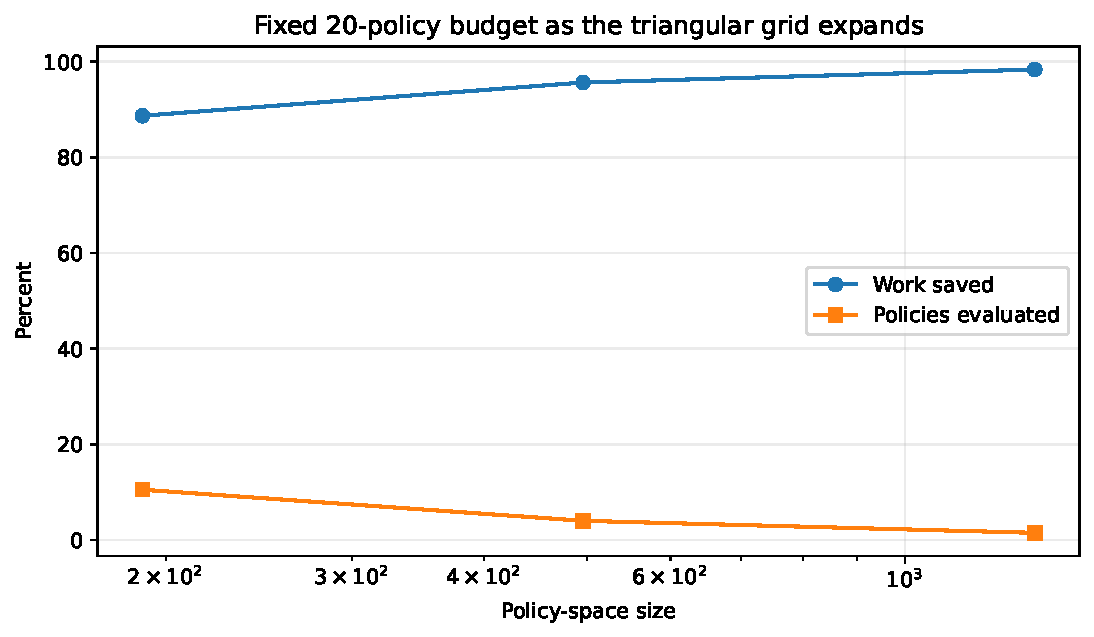
\includegraphics[width=.72\linewidth]{figures/policy_scaling.pdf}
\caption{Work reduction and evaluated fraction under a fixed 20-policy
high-fidelity budget. The experiment is a computational scaling check rather
than a reliability study.}
\label{fig:scaling}
\end{figure}

The result demonstrates that the evaluated fraction decreases rapidly as the
triangular grid grows. It does not show that a constant 20-policy budget will
remain adequate for every larger problem or scenario family.

\subsection{Practical reference policies}

Using one prespecified DR-BGS initialization, the selected policies improve
the median holdout objective by 30.96\% relative to local-only execution,
13.28\% relative to \((0.5K,0.5K)\), and 11.79\% relative to the fixed
\((0.5K,0.4K)\) deadband. DR-BGS is better in all 36 scenarios for these
three comparisons.

Against the strongest diagonal policy selected on training data, the median
difference is \(-0.38\%\), and DR-BGS is better in 41.67\% of scenarios.
Strict hysteresis is therefore not uniformly superior to the strongest
single-threshold alternative.

\begin{figure}[h]
\centering
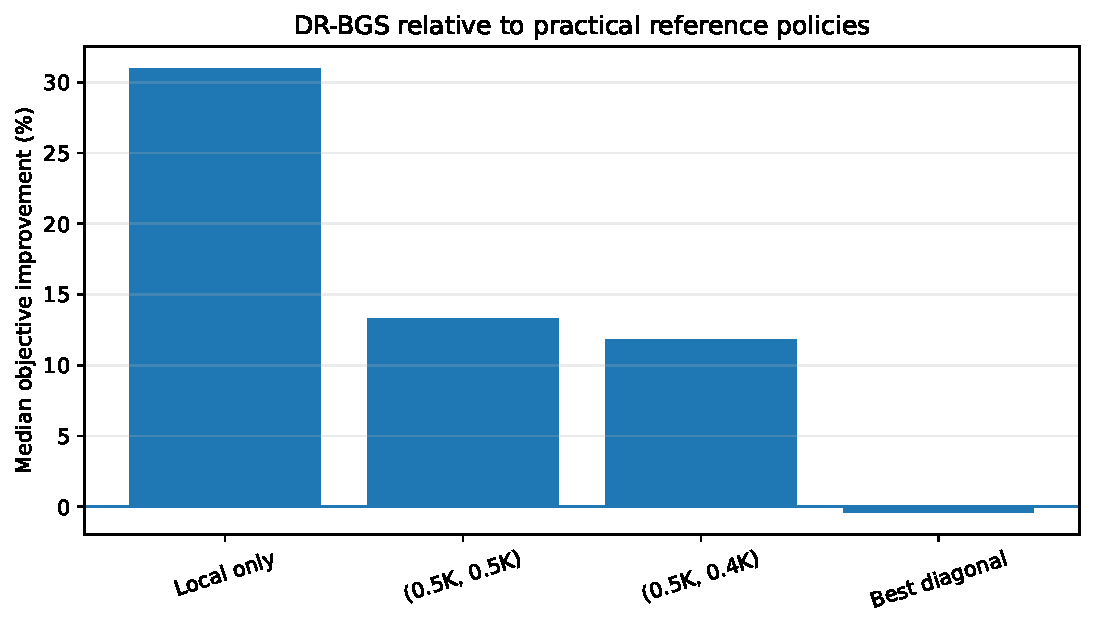
\includegraphics[width=.72\linewidth]{figures/practical_baselines.pdf}
\caption{Median objective improvement of DR-BGS relative to practical
reference policies. Negative improvement against the strongest diagonal
policy indicates no universal strict-hysteresis advantage.}
\label{fig:baselines}
\end{figure}

\subsection{Activation-delay sensitivity}

A delay-aware diffusion design evaluated under the actual-delay jump model
improves over a policy selected under a near-instantaneous activation
assumption by 3.04\% in the median, 12.82\% at the 90th percentile, and
17.69\% at maximum.

\begin{table}[h]
\centering
\small
\caption{Benefit of delay-aware policy design under the actual-delay model.}
\label{tab:delay}
\begin{tabular}{lr}
\toprule
Summary statistic & Objective improvement\\
\midrule
Median & 3.04\%\\
90th percentile & 12.82\%\\
Maximum & 17.69\%\\
\bottomrule
\end{tabular}
\end{table}

The median effect is moderate, but the upper tail shows that ignoring startup
delay can materially alter policy quality in some regimes.

\subsection{Incremental value of strict hysteresis}

Using complete holdout surfaces as a retrospective diagnostic, the best
strict-hysteresis policy improves over the best diagonal policy in 41.67\% of
the original 36 scenarios. The median gain is zero, the 90th percentile is
1.03\%, and the maximum is 2.85\%.

\begin{figure}[h]
\centering
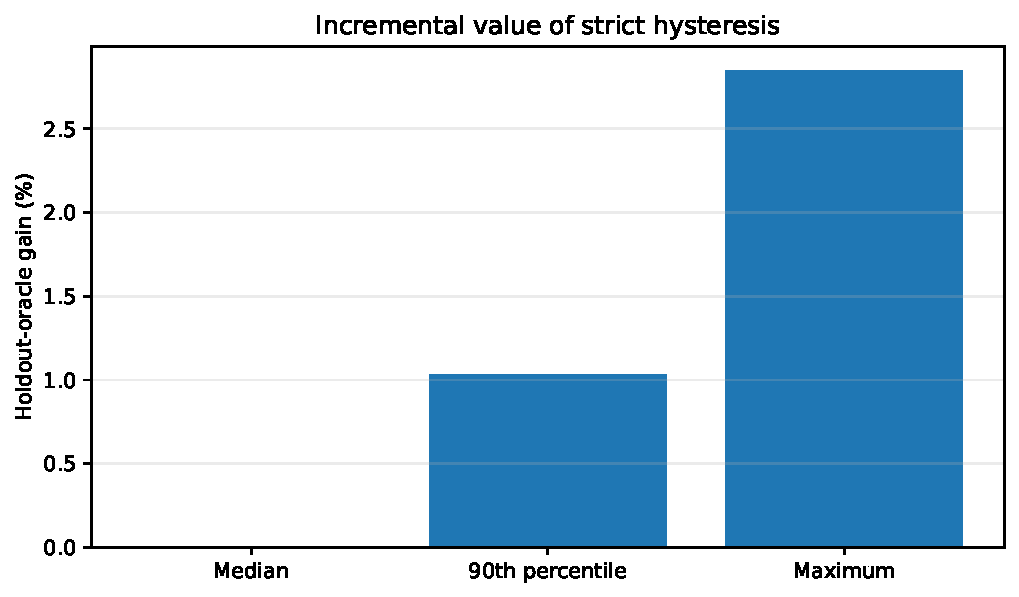
\includegraphics[width=.68\linewidth]{figures/hysteresis_gain.pdf}
\caption{Summary of incremental holdout-oracle gain from admitting a separate
release threshold.}
\label{fig:hysteresis}
\end{figure}

The expanded policy space remains useful because it includes both diagonal
and strict-hysteresis alternatives and permits data-driven selection. The
result does not support a universal superiority claim.

\subsection{Pareto and minimax-regret policies}

The holdout metrics \((W,B_H,B_L,R_C)\) are normalized within scenario. A
simplex grid of 286 weight vectors with step 0.1, augmented by equal weights,
produces 287 stakeholder profiles. For policy \(a\) and profile \(w\), let
\(C_w(a)\) be the normalized weighted cost and \(C_w^\star\) its optimum.
The minimax-regret policy is
\[
a_{\rm MR}
\in
\arg\min_a
\max_w
\left[
C_w(a)-C_w^\star
\right].
\]

Across 95 scenarios, the median Pareto set contains 118 of 190 policies, and
the median number of distinct profile-optimal policies is 13. The minimax
policy differs from the equal-weight policy in every scenario and is Pareto
efficient on the point-estimate surfaces. Its median maximum normalized
regret is 0.462, compared with 1.000 for the equal-weight policy, a reduction
of 52.63\%. The compromise pays a median normalized penalty of 0.174 under
equal weights.

\begin{figure}[h]
\centering
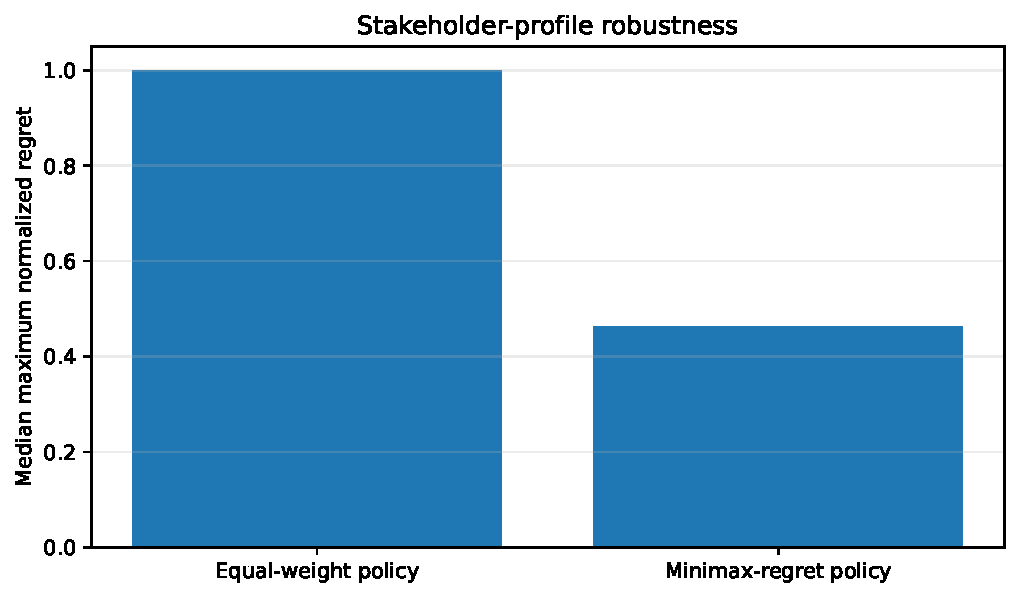
\includegraphics[width=.66\linewidth]{figures/minimax_regret.pdf}
\caption{Median maximum normalized regret over 287 stakeholder profiles.}
\label{fig:minimax}
\end{figure}

In the median scenario, the minimax policy is more than 5\% above the
profile optimum for 83.62\% of profiles, compared with 19.51\% for the
equal-weight policy. These results use point estimates and do not include
uncertainty in Pareto dominance.

\FloatBarrier

\section{Service-law calibration detail}
\label{sec:calibration}

\subsection{Measurement role}

The local-service law is
\[
s_n(x)=s_{0,n}\exp(-\beta_nx/K).
\]
The calibration tests whether an exponential decline is a plausible
reduced-order description over an observed hardware range. It does not
validate the complete threshold controller.

The principal measurements use Qwen2.5-7B served with vLLM on an NVIDIA RTX
3090 at six concurrency levels. The predictor is mean vLLM GPU KV-cache
usage, and the response is effective per-stream decode rate. Hardware,
serving configuration, model, request generation, and metric definitions are
held fixed across the six levels.

\subsection{Fit and cross-validation}

The fitted law is
\[
\widehat\mu(z)
=
53.6138\exp(-0.034451z).
\]
It gives
\[
R^2=0.9961,
\qquad
\operatorname{RMSE}=0.789\ {\rm tokens/s}.
\]
Because the in-sample \(R^2\) is based on the same six operating levels used
for fitting, leave-one-level-out refitting is also reported. Its prediction
RMSE is 1.299 tokens/s.

\begin{figure}[h]
\centering
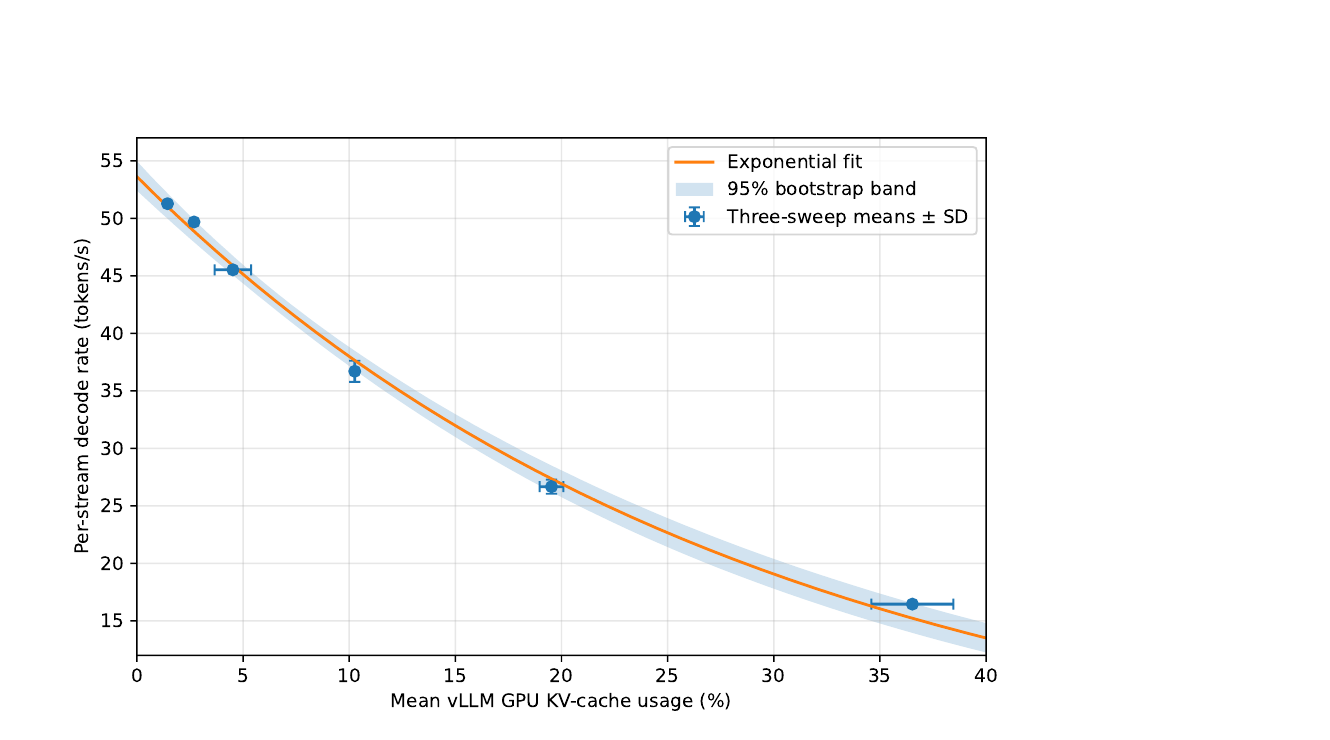
\includegraphics[width=.72\linewidth]{figures/service_law_fit.png}
\caption{Measured effective decode rate and fitted exponential law for
Qwen2.5-7B on the RTX 3090.}
\label{fig:calibration}
\end{figure}

\subsection{Bootstrap and simulator mapping}

A 20,000-draw bootstrap gives a normalized observed-range degradation
interval of
\[
1.159\leq\beta\leq1.358.
\]
The synthetic benchmark uses
\[
0.600\leq\beta\leq1.376,
\]
which deliberately includes slower degradation and additional structural
uncertainty. The fitted coefficient \(0.034451\) is not compared directly
with dimensionless \(\beta\) before mapping the measured \(z\)-range to the
normalized state \(x/K\).

RTX 4090 and Mistral measurements are retained as qualitative checks. They
show the same directional decline but are not pooled because their hardware,
model, or direct-telemetry protocols differ.

The calibration supports only three limited statements:

\begin{enumerate}
\item effective service declines as measured cache-related pressure rises;
\item an exponential law fits the principal RTX 3090 measurements over the
observed range; and
\item the simulation range contains the telemetry-derived estimates and
additional structural uncertainty.
\end{enumerate}

It does not establish coefficient transfer across GPUs or models, exact
physical meaning of \(X(t)\), or end-to-end controller validity.


\section{Retrospective analytical and model-form validation}
\label{sec:supp-validation}

This section documents a post hoc campaign performed after the primary study
results were known. It is not a preregistered or prospective replication.

\subsection{Independent optimizer implementation}

The public structural-anchor and Gaussian-process rules were reimplemented
from the archived algorithm description and applied directly to the 36
exhaustive policy surfaces.

\begin{table}[h]
\centering
\small
\caption{Independent optimizer reanalysis over 180 scenario--seed runs.}
\begin{tabular}{lrrrr}
\toprule
Method & Within 1\% & Within 5\% & Maximum excess & Exact recovery\\
\midrule
DR-BGS & 100.0\% & 100.0\% & 0.348\% & 88.9\%\\
Guarded GP & 100.0\% & 100.0\% & 0.878\% & 86.1\%\\
Standard GP & 95.6\% & 98.9\% & 7.220\% & 78.3\%\\
\bottomrule
\end{tabular}
\end{table}

The reimplementation reproduces the reported DR-BGS and guarded-GP worst
cases.

\subsection{Policy-surface ranking and absolute error}

Across 36 scenarios, the median diffusion/holdout Spearman correlation is
0.989, with scenario-bootstrap 95\% interval
0.977--0.992. Median Kendall correlation is 0.921,
and median top-20 overlap is 85.0\%. In contrast, median
scenario-level absolute objective error is 33.4\%.

\begin{figure}[h]
\centering
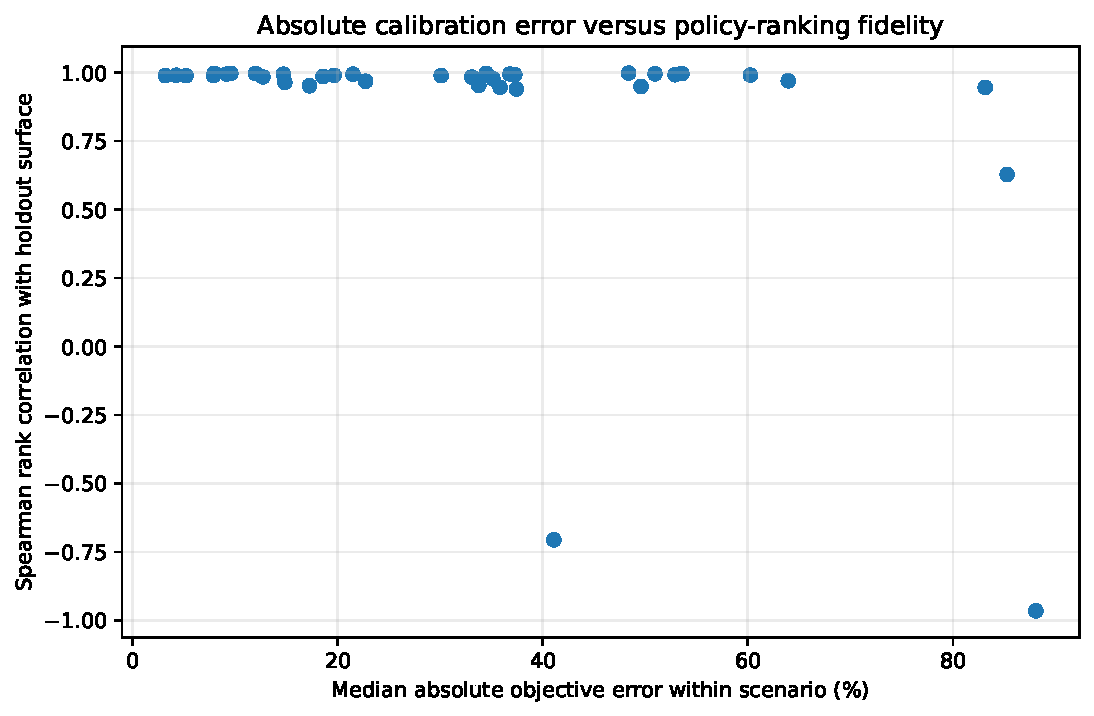
\includegraphics[width=.72\linewidth]{figures/surface_rank_vs_error.pdf}
\caption{Policy-ranking fidelity versus absolute objective error.}
\end{figure}

The diffusion-best policy exactly matches exhaustive training selection in
50.0\% of scenarios. Its 90th-percentile and maximum holdout
excesses are 5.68\% and 13.86\%, respectively. The diffusion
is therefore suitable as a trend but not as the sole policy selector.

\subsection{Jump-remainder and boundary indicators}

For Gamma jumps with mean \(m\) and coefficient of variation \(c\),
\[
\mathbb E[J^2]=m^2(1+c^2),
\qquad
\mathbb E[J^3]=m^3(1+c^2)(1+2c^2).
\]
The interior Taylor remainder satisfies
\[
|R_3f|
\leq
\frac{M_3}{6}\|f'''\|_\infty,
\]
and the capacity-scaled ratio of third- to second-order coefficients is
\(M_3/(3KM_2)\). Its median is 0.075 and its maximum is 0.216.
The median protected-jump overflow probability within the final 5\% of
capacity is 0.484.

\begin{figure}[h]
\centering
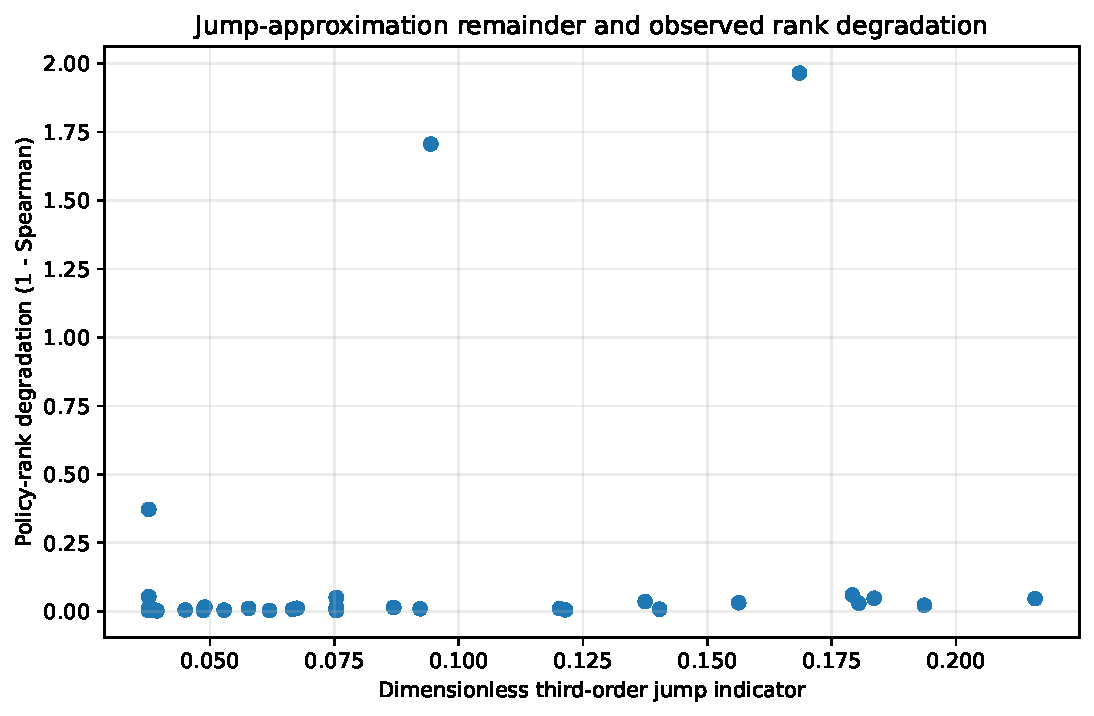
\includegraphics[width=.70\linewidth]{figures/jump_indicator.pdf}
\caption{Third-order jump indicator and policy-rank degradation.}
\end{figure}

Jump coefficient of variation and the third-order indicator have Spearman
associations 0.438 and 0.348 with rank degradation. These are diagnostic
associations rather than causal estimates.

\subsection{Direct service-law model comparison}

The direct RTX 3090 fit is
\[
\widehat\mu(z)
=
53.6138
\exp(-0.034451z).
\]
Its RMSE is 0.789 tokens/s, \(R^2=0.9961\), AICc 5.16,
and leave-one-level-out RMSE 1.299 tokens/s. The 10,000-draw
bootstrap intervals are 53.376--53.857 for the intercept and
0.03326--0.03567 for the decay coefficient.

\subsection{Cross-hardware and cross-model transport}

\begin{figure}[h]
\centering
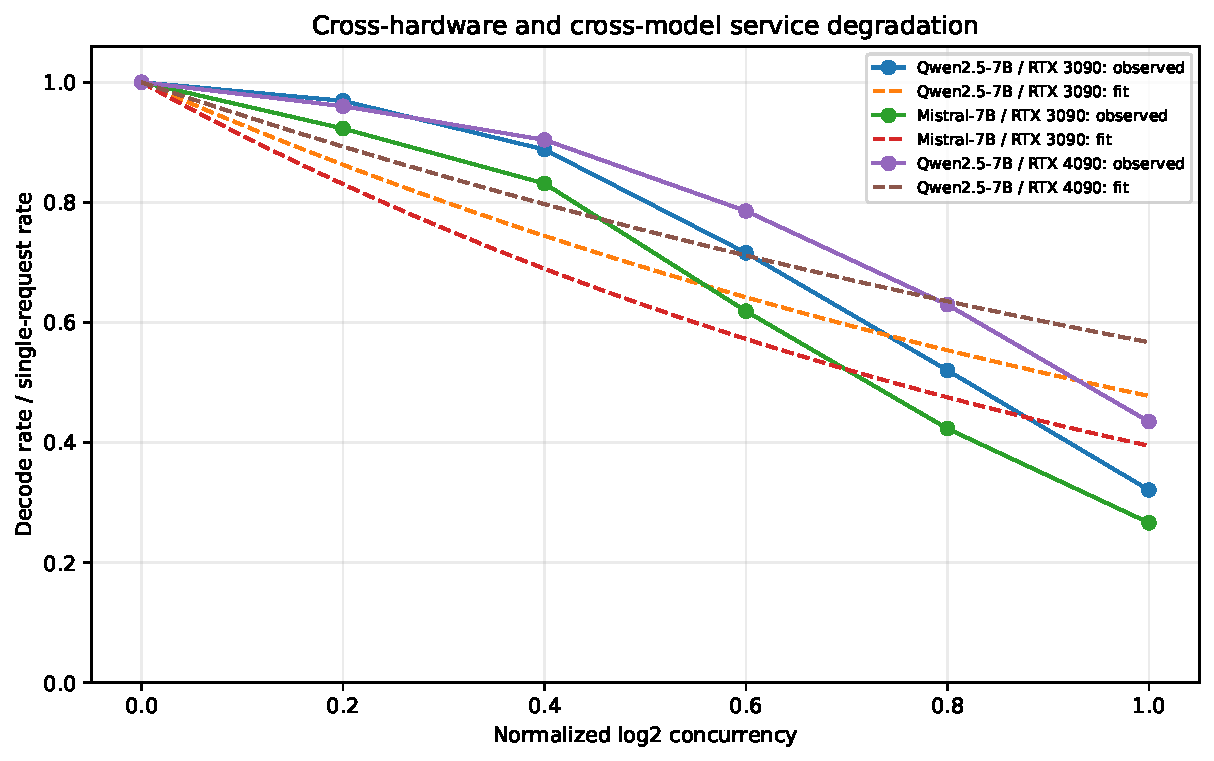
\includegraphics[width=.80\linewidth]{figures/cross_hardware_transport.pdf}
\caption{Normalized service curves and domain-specific exponential fits.}
\end{figure}

All primary curves are strictly decreasing. Pairwise normalized-curve RMSE
ranges from 0.067 to 0.133. Leave-one-domain-out RMSE ranges from
0.103 to 0.131. The shared exponential \(R^2\) is 0.812.
A common decline shape is supported, but a common coefficient is not.

\subsection{Low-fidelity model-form stress}

\begin{figure}[h]
\centering
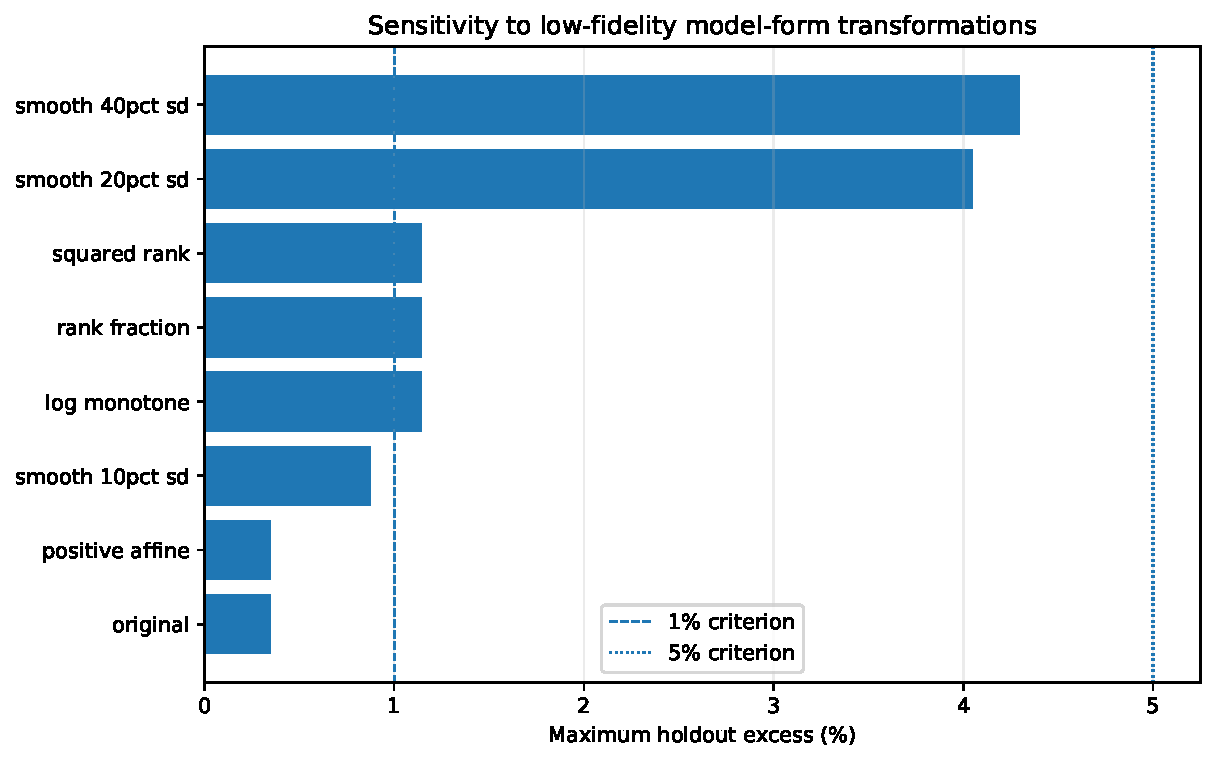
\includegraphics[width=.78\linewidth]{figures/model_form_stress.pdf}
\caption{Maximum holdout excess after low-fidelity transformations.}
\end{figure}

Every tested transformation retains a 100\% within-5\% rate. Positive affine
transformation is invariant. The strongest smooth perturbation has median
Kendall correlation 0.944 and maximum excess
4.29\%. These are heuristic sensitivity tests rather than physical
service-model substitutions.

\subsection{Independent solver triangulation}

Eighteen unique policy cases from six scenario types were solved with an
independently implemented CTMC at 161 and 321 grid points and with a separate
Euler--Maruyama reflected-diffusion simulation.

\begin{figure}[h]
\centering
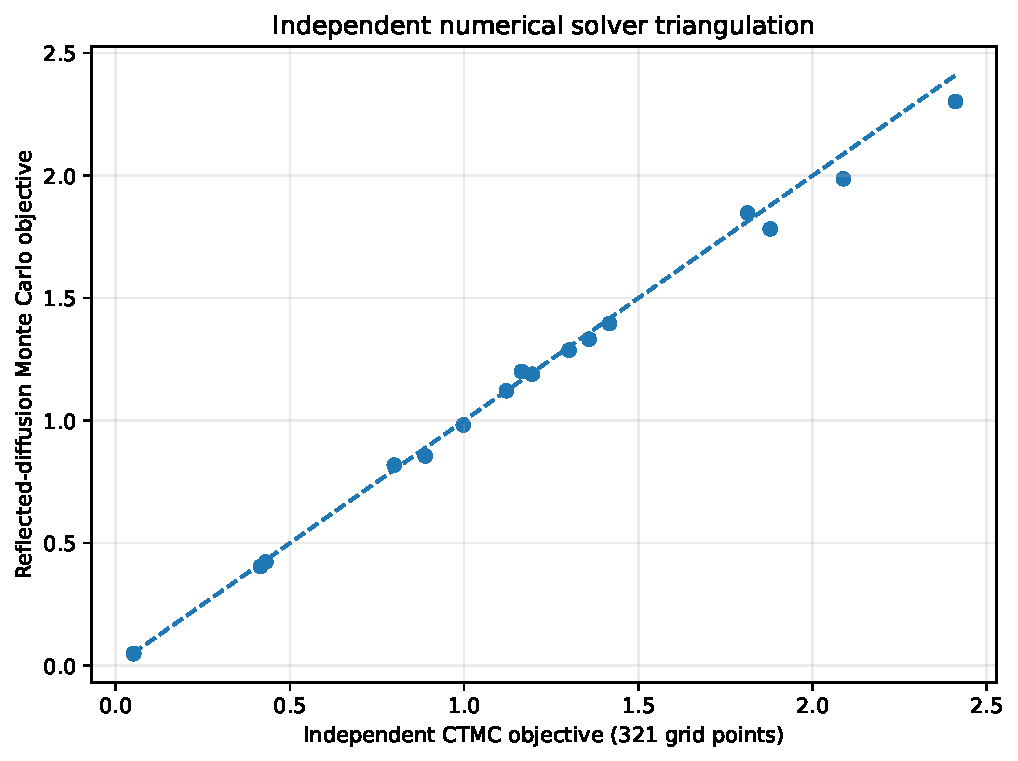
\includegraphics[width=.70\linewidth]{figures/solver_triangulation.pdf}
\caption{Independent CTMC and stochastic reflected-diffusion objectives.}
\end{figure}

The independent 161-point CTMC differs from the archived 161-point
objective by median below $10^{-4}$\% and maximum 0.608\%. The 161-to-321 grid change is
median 1.17\% and maximum 2.25\%. The Monte Carlo/321-point
CTMC difference is median 2.52\%, 90th percentile 4.94\%, and
maximum 6.67\%. Median policy-rank Spearman is 1.0, and
the best policy agrees in 83.3\% of scenario comparisons.

The campaign strengthens model and implementation validity but does not
remove the absence of end-to-end controller execution on real infrastructure.

\section{Reproducibility map}
\label{sec:reproducibility}

The repository archive contains:

\begin{itemize}
\item simulator and optimizer code;
\item exhaustive 190-policy training and holdout surfaces;
\item comparator and ablation outputs;
\item trace transformation and replay scripts;
\item original and seven-day protocol locks;
\item fresh low-load confirmation outputs;
\item source-trace provenance hashes;
\item calibration data and scripts;
\item figures, result tables, and checksum manifests; and
\item audit scripts and human-readable reports.
\end{itemize}

The code, data, audit artifacts, and reproducibility materials are available
at
\[
\href{https://doi.org/10.5281/zenodo.21434924}
{\texttt{doi:10.5281/zenodo.21434924}}.
\]
The corresponding GitHub repository and release are
\[
\href{https://github.com/AMD-Aljohani/dr-bgs-llm-routing}
{\texttt{AMD-Aljohani/dr-bgs-llm-routing}}
\]
and
\[
\href{https://github.com/AMD-Aljohani/dr-bgs-llm-routing/releases/tag/v1.1.0}
{\texttt{v1.1.0}}.
\]

Immutable provenance checks validate tracked lock metadata, locked-input
hashes, required scientific artifacts, and the repository checksum manifest.
The repository does not claim that historical filesystem modification times
prove execution chronology.

\section{Supplementary interpretation}

The expanded material supports the same restrained conclusion as the main
manuscript. DR-BGS is a problem-specific simulation-optimization workflow,
not a general safety theorem. Structural search coverage contributes most of
the finite-budget reliability, while the diffusion residual provides an
additional ranking improvement. Independent later-pool risk evaluation can
abstain even when nomination is near exhaustive selection. Exhaustive
high-load evaluation and enlarged certification batches show that the
reported abstention is not explained by a missed tested policy or the
original sample size. Positive low-load confirmation identifies a modeled
operating envelope rather than a recommended production configuration.

\PublishersNote{}
\end{document}
